\documentclass[11pt,a4paper]{article}
\usepackage[margin=1in]{geometry}
\usepackage{amsmath,amssymb}
\usepackage{graphicx}
\usepackage{enumitem}
\usepackage{tcolorbox}
\usepackage{array}
\usepackage{multirow}
\usepackage{tikz}
\usepackage{xcolor}
\usepackage{hyperref}
\usetikzlibrary{positioning,arrows.meta,shapes,calc}

% Colors matching educational scheme
\definecolor{codegreen}{rgb}{0,0.6,0}
\definecolor{codegray}{rgb}{0.5,0.5,0.5}
\definecolor{codepurple}{rgb}{0.58,0,0.82}
\definecolor{backcolour}{rgb}{0.95,0.95,0.92}

% Custom commands
\newcommand{\highlight}[1]{\textbf{\color{blue}#1}}
\newcommand{\answer}[1]{\underline{\hspace{#1}}}
\newcommand{\checkbox}{$\Box$}

% Environment definitions
\newtcolorbox{exercise}[1][]{
    colback=blue!5!white,
    colframe=blue!75!black,
    title=#1,
    fonttitle=\bfseries
}

\newtcolorbox{checkpoint}[1][]{
    colback=yellow!10!white,
    colframe=orange!75!black,
    title=Checkpoint,
    fonttitle=\bfseries
}

\newtcolorbox{discovery}[1][]{
    colback=green!5!white,
    colframe=green!75!black,
    title=Discovery Moment,
    fonttitle=\bfseries
}

\newtcolorbox{think}[1][]{
    colback=purple!5!white,
    colframe=purple!75!black,
    title=Think About It,
    fonttitle=\bfseries
}

\newtcolorbox{realworld}[1][]{
    colback=orange!5!white,
    colframe=orange!75!black,
    title=Real World Application,
    fonttitle=\bfseries
}

\newtcolorbox{warning}[1][]{
    colback=red!5!white,
    colframe=red!75!black,
    title=Common Pitfall,
    fonttitle=\bfseries
}

% Title and header
\title{\textbf{Week 4: Sequence-to-Sequence Models}\\
\large Post-Class Learning Verification\\
\vspace{0.5em}
\large \textit{From Fixed-Length Prison to Variable-Length Freedom}}
\author{NLP Course 2025 - Assessment}
\date{}

\begin{document}
\maketitle

\noindent\textbf{Time Required:} 45-60 minutes\\
\textbf{Purpose:} Verify and deepen your understanding of seq2seq models after completing the lab\\
\textbf{Format:} Conceptual problems, implementation questions, and real-world applications

\begin{checkpoint}
\textbf{Before Starting:} You should have completed the Week 4 lab and understood:
\begin{itemize}
    \item Why variable-length sequences need special handling
    \item The encoder-decoder architecture
    \item The information bottleneck problem
    \item How attention mechanism works
    \item Beam search for sequence generation
\end{itemize}
\end{checkpoint}

\hrule
\vspace{1em}

\section*{Part A: Conceptual Understanding \hfill (25 minutes)}

\subsection*{A1: The Variable-Length Problem (5 minutes)}

\begin{exercise}[Understanding the Core Challenge]
\textbf{Question 1:} Explain why traditional RNNs cannot handle translation tasks effectively.

\vspace{3cm}

\textbf{Question 2:} Consider these translation pairs. Circle the fundamental problem:
\begin{itemize}
    \item English: "How are you?" (3 words) → Spanish: "¿Cómo estás?" (2 words)
    \item English: "Thank you" (2 words) → German: "Vielen Dank" (2 words)  
    \item English: "Good morning" (2 words) → Japanese: "Ohayou gozaimasu" (2 words)
\end{itemize}

\begin{itemize}
    \item[\checkbox] Different word counts between languages
    \item[\checkbox] RNNs can only produce one output per input
    \item[\checkbox] No shared vocabulary between languages
    \item[\checkbox] Grammar structures are too different
\end{itemize}

\textbf{Question 3:} List three real-world applications where variable-length input/output is essential:

1. \answer{8cm}

2. \answer{8cm}

3. \answer{8cm}
\end{exercise}

\subsection*{A2: Encoder-Decoder Architecture (8 minutes)}

\begin{exercise}[Understanding the Solution]
\textbf{Question 1:} Draw and label the encoder-decoder architecture for translating "The cat sleeps" → "Le chat dort":

\begin{center}
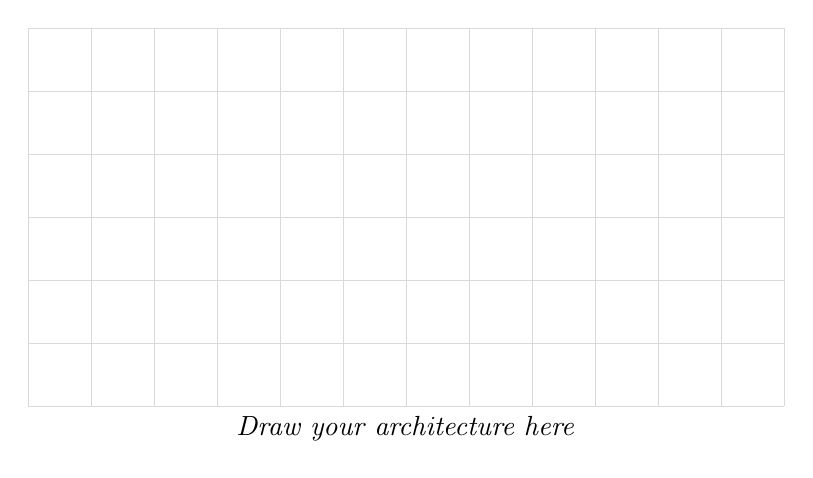
\begin{tikzpicture}[scale=0.8]
    % Grid for drawing
    \draw[gray!30] (0,0) grid (12,6);
    \node[below] at (6,0) {\textit{Draw your architecture here}};
\end{tikzpicture}
\end{center}

\textbf{Question 2:} Complete the mathematical description:

\begin{itemize}
    \item Encoder equations: $h_t = $ \answer{5cm}
    \item Context vector: $c = $ \answer{5cm}
    \item Decoder equations: $s_t = $ \answer{5cm}
    \item Output probability: $P(y_t | \ldots) = $ \answer{5cm}
\end{itemize}

\textbf{Question 3:} Why is the context vector a "bottleneck"?

\vspace{3cm}

\textbf{Question 4:} If your encoder has 128 hidden units and processes a 20-word sentence, what is the size of:
\begin{itemize}
    \item Context vector: \answer{3cm} dimensions
    \item Total encoder information: \answer{3cm} dimensions  
    \item Information compression ratio: \answer{3cm}
\end{itemize}
\end{exercise}

\subsection*{A3: Attention Mechanism Deep Dive (8 minutes)}

\begin{exercise}[Attention Mathematics and Intuition]
\textbf{Question 1:} Complete the attention mechanism steps:

Step 1: Compute alignment scores: $e_{t,i} = $ \answer{6cm}

Step 2: Normalize with softmax: $\alpha_{t,i} = $ \answer{6cm}

Step 3: Compute context vector: $c_t = $ \answer{6cm}

\textbf{Question 2:} Given these simplified encoder states and decoder state:
\begin{itemize}
    \item $h_1 = [0.5, 0.2]$ (word: "The")
    \item $h_2 = [0.8, 0.1]$ (word: "cat") 
    \item $h_3 = [0.3, 0.7]$ (word: "sleeps")
    \item $s_t = [0.7, 0.3]$ (generating French word)
\end{itemize}

Calculate dot-product attention weights:
\begin{itemize}
    \item $e_{t,1} = h_1 \cdot s_t = $ \answer{3cm}
    \item $e_{t,2} = h_2 \cdot s_t = $ \answer{3cm}  
    \item $e_{t,3} = h_3 \cdot s_t = $ \answer{3cm}
\end{itemize}

Which word gets highest attention? \answer{3cm}

\textbf{Question 3:} Attention visualization interpretation. If you see this attention pattern:

\begin{center}
\begin{tabular}{|l|c|c|c|c|}
\hline
\textbf{French} & \textbf{The} & \textbf{black} & \textbf{cat} & \textbf{sleeps} \\
\hline
Le & 0.8 & 0.1 & 0.1 & 0.0 \\
\hline
chat & 0.1 & 0.1 & 0.8 & 0.0 \\
\hline
noir & 0.0 & 0.9 & 0.1 & 0.0 \\
\hline
dort & 0.0 & 0.0 & 0.1 & 0.9 \\
\hline
\end{tabular}
\end{center}

What pattern do you observe? \answer{8cm}

Why is this good for translation? \answer{8cm}
\end{exercise}

\subsection*{A4: Beam Search Strategy (4 minutes)}

\begin{exercise}[Search and Generation]
\textbf{Question 1:} Why can't we just use greedy search (always pick highest probability word)?

\vspace{2cm}

\textbf{Question 2:} Complete this beam search example (beam size = 2):

Starting with "START", expand to first word:
\begin{itemize}
    \item P("Le" | START) = 0.6
    \item P("Un" | START) = 0.3
    \item P("La" | START) = 0.1
\end{itemize}

Keep top 2: \answer{4cm} and \answer{4cm}

Expand "Le" to second word:
\begin{itemize}
    \item P("chat" | Le) = 0.8 → Total: \answer{3cm}
    \item P("chien" | Le) = 0.2 → Total: \answer{3cm}
\end{itemize}

Expand "Un" to second word:
\begin{itemize}
    \item P("chat" | Un) = 0.7 → Total: \answer{3cm}
    \item P("chien" | Un) = 0.3 → Total: \answer{3cm}
\end{itemize}

Final top 2 sequences: \answer{6cm} and \answer{6cm}

\textbf{Question 3:} What happens to beam search quality vs. beam size?

Beam size 1: \answer{5cm}

Beam size 100: \answer{5cm}

Optimal beam size (typical): \answer{3cm}
\end{exercise}

\newpage

\section*{Part B: Implementation and Code Understanding \hfill (15 minutes)}

\subsection*{B1: Code Analysis (8 minutes)}

\begin{exercise}[PyTorch Implementation]
\textbf{Question 1:} Analyze this encoder code. Fill in the missing dimensions:

\begin{verbatim}
class Seq2SeqEncoder(nn.Module):
    def __init__(self, vocab_size=5000, embed_size=128, hidden_size=256):
        self.embedding = nn.Embedding(vocab_size, embed_size)
        self.lstm = nn.LSTM(embed_size, hidden_size, batch_first=True)
    
    def forward(self, x):  # x shape: [batch_size, seq_len]
        embedded = self.embedding(x)  # shape: [______, ______, ______]
        output, (h_n, c_n) = self.lstm(embedded)
        return h_n, c_n  # shapes: [______, ______], [______, ______]
\end{verbatim}

Fill in the shapes:
\begin{itemize}
    \item embedded shape: [\answer{2cm}, \answer{2cm}, \answer{2cm}]
    \item h\_n shape: [\answer{2cm}, \answer{2cm}]
    \item c\_n shape: [\answer{2cm}, \answer{2cm}]
\end{itemize}

\textbf{Question 2:} What's wrong with this attention implementation?

\begin{verbatim}
def attention(decoder_hidden, encoder_outputs):
    scores = torch.matmul(decoder_hidden, encoder_outputs.T)
    weights = F.softmax(scores, dim=1)
    context = torch.sum(weights * encoder_outputs, dim=1)
    return context
\end{verbatim}

Problem: \answer{8cm}

Fix: \answer{8cm}

\textbf{Question 3:} Complete this beam search pseudocode:

\begin{verbatim}
def beam_search(model, input_seq, beam_size=4, max_length=20):
    beams = [{"sequence": [START_TOKEN], "score": 0.0}]
    
    for step in range(max_length):
        candidates = []
        for beam in beams:
            if beam["sequence"][-1] == END_TOKEN:
                candidates.append(beam)
                continue
            
            # Get next word probabilities
            probs = model.predict_next(beam["sequence"])
            
            # Expand beam
            for word, prob in probs.top_k(beam_size):
                new_score = ___________________
                new_sequence = ______________
                candidates.append({"sequence": new_sequence, "score": new_score})
        
        # Keep top beam_size candidates
        beams = sorted(candidates, key=lambda x: x["score"])[:______]
    
    return beams[0]["sequence"]
\end{verbatim}

Fill in the blanks:
\begin{itemize}
    \item new\_score = \answer{5cm}
    \item new\_sequence = \answer{5cm}
    \item Keep top: \answer{2cm}
\end{itemize}
\end{exercise}

\subsection*{B2: Training Insights (7 minutes)}

\begin{exercise}[Training Process]
\textbf{Question 1:} What is "teacher forcing" and why do we use it during training?

Definition: \answer{8cm}

Why use it: \answer{8cm}

What problem does it cause: \answer{8cm}

\textbf{Question 2:} Loss function analysis. Given these target and predicted sequences:

Target: ["Le", "chat", "dort", "<EOS>"]
Predicted logits for each position:
\begin{itemize}
    \item Position 1: P("Le")=0.8, P("Un")=0.15, P("La")=0.05
    \item Position 2: P("chat")=0.9, P("chien")=0.07, P("oiseau")=0.03
    \item Position 3: P("dort")=0.6, P("mange")=0.3, P("court")=0.1
    \item Position 4: P("<EOS>")=0.95, P("bien")=0.03, P("mal")=0.02
\end{itemize}

Calculate the cross-entropy loss:
\begin{itemize}
    \item Position 1 loss: $-\log(0.8) = $ \answer{3cm}
    \item Position 2 loss: $-\log(0.9) = $ \answer{3cm}
    \item Position 3 loss: $-\log(0.6) = $ \answer{3cm}
    \item Position 4 loss: $-\log(0.95) = $ \answer{3cm}
    \item Total loss: \answer{3cm}
\end{itemize}

\textbf{Question 3:} Why might attention weights look random at the start of training?

\vspace{2cm}

What should happen to attention weights as training progresses?

\vspace{2cm}
\end{exercise}

\newpage

\section*{Part C: Real-World Applications \hfill (12 minutes)}

\subsection*{C1: Modern Applications Analysis (6 minutes)}

\begin{exercise}[2024 Industry Applications]
\textbf{Question 1:} Map these modern systems to seq2seq components:

\begin{center}
\begin{tabular}{|l|l|l|}
\hline
\textbf{Application} & \textbf{Input} & \textbf{Output} \\
\hline
Google Translate & & \\
\hline
GitHub Copilot & & \\
\hline
Email Summarization & & \\
\hline
Text-to-SQL & & \\
\hline
Chatbot Response & & \\
\hline
\end{tabular}
\end{center}

\textbf{Question 2:} Which of these would benefit most from attention mechanism?
\begin{itemize}
    \item[\checkbox] Translating short phrases (3-5 words)
    \item[\checkbox] Translating technical documents (500+ words)
    \item[\checkbox] Generating code from one-line comments
    \item[\checkbox] Summarizing research papers
    \item[\checkbox] Converting speech to text
\end{itemize}

Explain your top choice: \answer{8cm}

\textbf{Question 3:} Compare 2014 vs 2024 seq2seq capabilities:

\begin{center}
\begin{tabular}{|l|l|l|}
\hline
\textbf{Aspect} & \textbf{2014 (Original)} & \textbf{2024 (Modern)} \\
\hline
Max input length & & \\
\hline
Translation quality & & \\
\hline
Inference speed & & \\
\hline
Model size & & \\
\hline
Applications & & \\
\hline
\end{tabular}
\end{center}
\end{exercise}

\subsection*{C2: System Design Challenge (6 minutes)}

\begin{exercise}[Building Real Systems]
\textbf{Question 1:} Design a meeting summarization system:

\textbf{Input:} 2-hour meeting transcript (5000 words)
\textbf{Output:} Key points and action items (200 words)

Your architecture:
\begin{itemize}
    \item Preprocessing: \answer{8cm}
    \item Encoder design: \answer{8cm}
    \item Attention strategy: \answer{8cm}
    \item Decoder design: \answer{8cm}
    \item Post-processing: \answer{8cm}
\end{itemize}

\textbf{Question 2:} Code comment to function generator:

\textbf{Input:} "Function to calculate fibonacci numbers up to n"
\textbf{Output:} Complete Python function

What challenges would this face?
\begin{enumerate}
    \item \answer{8cm}
    \item \answer{8cm}
    \item \answer{8cm}
\end{enumerate}

How would attention help? \answer{8cm}

\textbf{Question 3:} Multilingual customer support system:

Requirements:
\begin{itemize}
    \item Input: Customer query in any of 10 languages
    \item Output: Response in same language as input
    \item Must handle domain-specific terminology
\end{itemize}

Design approach:
\begin{itemize}
    \item Language detection: \answer{6cm}
    \item Translation pipeline: \answer{6cm}
    \item Response generation: \answer{6cm}
    \item Quality assurance: \answer{6cm}
\end{itemize}
\end{exercise}

\newpage

\section*{Part D: Critical Thinking and Extensions \hfill (8 minutes)}

\subsection*{D1: Problem Solving (4 minutes)}

\begin{warning}
Real challenges you might encounter in production:
\end{warning}

\begin{exercise}[Debugging and Optimization]
\textbf{Scenario 1:} Your seq2seq translator produces repetitive output: "The cat the cat the cat sleeps"

Possible causes:
\begin{itemize}
    \item[\checkbox] Attention weights are too uniform
    \item[\checkbox] Beam search beam size too small
    \item[\checkbox] Training data has repetitive patterns
    \item[\checkbox] Learning rate too high
    \item[\checkbox] Decoder getting stuck in local optima
\end{itemize}

Best solution: \answer{8cm}

\textbf{Scenario 2:} Translation quality drops drastically for sentences longer than 20 words.

Root cause: \answer{8cm}

Solution strategy: \answer{8cm}

\textbf{Scenario 3:} Your model works great on formal text but fails on casual social media language.

Why this happens: \answer{8cm}

How to fix: \answer{8cm}
\end{exercise}

\subsection*{D2: Future Connections (4 minutes)}

\begin{think}
\textbf{Connecting to Advanced Topics:}

\textbf{Question 1:} How do Transformers (next week) improve on seq2seq?

Key improvements:
\begin{enumerate}
    \item \answer{8cm}
    \item \answer{8cm}
    \item \answer{8cm}
\end{enumerate}

\textbf{Question 2:} Modern large language models (ChatGPT, GPT-4) use modified seq2seq principles. What's different?

Architectural changes: \answer{8cm}

Scale differences: \answer{8cm}

Training approach: \answer{8cm}

\textbf{Question 3:} Beyond text, what other sequence-to-sequence problems exist?

\begin{itemize}
    \item Audio domain: \answer{6cm}
    \item Video domain: \answer{6cm}
    \item Scientific domain: \answer{6cm}
    \item Creative domain: \answer{6cm}
\end{itemize}
\end{think}

\hrule
\vspace{1em}

\section*{Self-Assessment and Next Steps}

\begin{checkpoint}
\textbf{Check your understanding level:}
\begin{itemize}
    \item[\checkbox] I can explain why seq2seq was needed (vs fixed-length RNNs)
    \item[\checkbox] I understand the encoder-decoder architecture completely
    \item[\checkbox] I can describe the information bottleneck problem
    \item[\checkbox] I can explain how attention solves the bottleneck
    \item[\checkbox] I can implement attention mechanism from scratch
    \item[\checkbox] I understand beam search vs greedy search trade-offs
    \item[\checkbox] I can design seq2seq systems for real applications
    \item[\checkbox] I see the connection to modern transformer models
\end{itemize}
\end{checkpoint}

\begin{realworld}
\textbf{Industry Relevance Check:}
Rate your confidence (1-5) for these career-relevant skills:
\begin{itemize}
    \item Building translation systems: \answer{2cm}
    \item Designing text summarization: \answer{2cm}
    \item Code generation tools: \answer{2cm}
    \item Conversational AI systems: \answer{2cm}
    \item Understanding modern LLM architecture: \answer{2cm}
\end{itemize}
\end{realworld}

\vspace{1em}

\textbf{Areas needing review:} \answer{10cm}

\textbf{Most interesting discovery:} \answer{10cm}

\textbf{Connection to your projects/interests:} \answer{10cm}

\hrule
\vspace{1em}

\section*{Next Steps}

\textbf{Immediate review:} Focus on areas where you scored below 3/5

\textbf{Hands-on practice:} 
\begin{itemize}
    \item Implement seq2seq from scratch in your preferred framework
    \item Try the model on a different language pair
    \item Experiment with different attention mechanisms
    \item Build a simple summarization system
\end{itemize}

\textbf{Preparation for Week 5:}
\begin{itemize}
    \item Review attention mechanism thoroughly
    \item Understand the limitations of RNN-based seq2seq
    \item Think about parallelization challenges
    \item Read "Attention Is All You Need" paper introduction
\end{itemize}

\vspace{2em}
\begin{center}
\textbf{--- End of Assessment ---}\\
\vspace{0.5em}
\textit{You're now ready to understand how Transformers revolutionized this field!}
\end{center}

\end{document}